\section{Results}
\label{sec:results}

\paragraph{The selection loss picks a checkpoint that never predicts \textsc{stop}.}
In every unweighted seed, the run beats the frequency-only baseline on the natural set, and the rule
selects update 160. Each selected checkpoint, however, predicts \textsc{stop} on $0/256$ selection
decisions and recalls $0/64$ of the balanced set's \textsc{stop} decisions.
Figure~\ref{fig:stop_moments} shows the three selection decisions at which the expert stops. On the
balanced set, each unweighted run's loss is worse than a uniform guess ($\ln 4$), although its accuracy
is better than chance ($0.25$). Class weighting improves
the balanced-set loss, accuracy, and \textsc{stop} recall in $3/3$ pairs, but worsens the
natural-set loss in $3/3$. Weighted \textsc{stop} recall is $12/64$, $1/64$, and $6/64$, so the
direction of the effect replicates across seeds but its size does not. All six existence gates fail
(Table~\ref{tab:seed-replication}). Figure~\ref{fig:blind_metric} plots the selection loss and the
number of predicted \textsc{stop}s over training. Figure~\ref{fig:metric_decomposition} breaks one
selected checkpoint's loss of $0.7373$ into its parts. Exact score ties go to
the lowest action ID, which is \textsc{stop} (Appendix~\ref{app:ties}).

\begin{figure}[t]
  \centering
  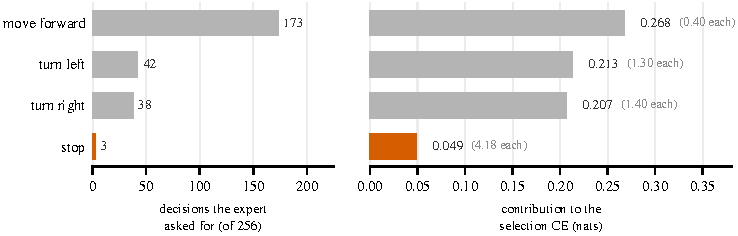
\includegraphics[width=\linewidth]{figures/p1_metric_decomposition.pdf}
  \caption{\textbf{Decomposition of the selection loss.} It is a mean over $256$ decisions, so
  each expert action contributes its own cross-entropy weighted by how often the expert asks for it.
  The four contributions sum to the reported $0.7373$ with no residual. \textsc{stop} has the worst
  per-decision cross-entropy, $4.18$ against $0.40$ for \textsc{move\_forward}, and this checkpoint
  never predicts it. At three decisions in $256$, that failure moves $6.6\%$ of the number. Update $160$,
  unweighted seed $20260826$; \textsc{stop}'s share is $3.5$--$6.2\%$ across the other five runs.}
  \label{fig:metric_decomposition}
\end{figure}

%
\begin{table}[t]
\centering
\small
\caption{Three-seed paired replication. Values are mean $\pm$ sample standard deviation; deltas are weighted minus unweighted. All seeds are reported. Natural CE is scored on the 640-decision natural set; selection CE, on the 256-decision selection set that picks each checkpoint (Figures~\ref{fig:metric_decomposition} and~\ref{fig:blind_metric}), is a different quantity.}
\label{tab:seed-replication}
\begin{tabular}{@{}lrrr@{}}
\toprule
Metric & Unweighted & Weighted & Paired delta \\
\midrule
Natural mean CE $\downarrow$ & 0.754 $\pm$ 0.012 & 0.955 $\pm$ 0.016 & $0.201 \pm 0.019$ \\
Balanced mean CE $\downarrow$ & 1.725 $\pm$ 0.117 & 1.452 $\pm$ 0.132 & $-0.273 \pm 0.223$ \\
Balanced accuracy $\uparrow$ & 0.332 $\pm$ 0.004 & 0.397 $\pm$ 0.038 & $0.065 \pm 0.042$ \\
Balanced \textsc{stop} recall $\uparrow$ & 0/64 in 3/3 seeds & 12/64, 1/64, 6/64 & $0.099 \pm 0.086$ \\
Existence gate & 0/3 passed & 0/3 passed & --- \\
\bottomrule
\end{tabular}
\end{table}


\paragraph{Success is zero for every selected checkpoint.}
Table~\ref{tab:closed-loop-behavior} summarizes the simulator runs, and
Appendix~\ref{app:closedloop} plots them. All six checkpoints obtain SR $0/61$, SPL $0$, and SDTW
$0$. Each $0/61$ is still consistent with a true success rate of up to $5.9\%$ (exact two-sided $95\%$
Clopper--Pearson interval, treating episodes as independent). Each also has OSR $1/61$, but from different episodes. Every unweighted checkpoint enters the
goal radius only on episode 562, and every weighted checkpoint only on episode 394. Episode 562
ends inside the radius, 2.356 m from the goal, after 480 decisions inside the radius without
\textsc{stop}. Episode 394 comes within 1.241 m of the goal, leaves the radius, and ends 4.513 m away
after 33 decisions inside it without \textsc{stop}. On these paths, a perfectly timed stop would have succeeded in at most $1$ of $61$ episodes. Most episodes fail because the policy never
reaches the goal, and on the one path that does reach it, the policy does not stop.

\paragraph{No checkpoint was shown to navigate better than the selected one.}
All $2{,}257$ episode runs of the 37 checkpoints completed (Table~\ref{tab:sweep},
Appendix~\ref{app:sweep}). The only checkpoint that succeeds is the untrained model, with
$1/61$ (episode 358, two-sided $95\%$ interval $0.04$--$8.8\%$). It also presses
\textsc{stop} $50$ times in other episodes. Each of the 36 trained checkpoints scores $0/61$. Of the
$213$ \textsc{stop} presses across all 37 checkpoints, one falls inside the goal radius. No
candidate reaches the preregistered bar against its run's selected checkpoint. The sweep was
designed to separate two explanations for the selected checkpoints' zero success. Either the loss
passed over a checkpoint that navigates, or no checkpoint it ranked was shown to navigate better
than its pick. It found no evidence for the first explanation, within the statistical power given
in Section~\ref{sec:limitations}. Re-executed in this sweep, the six selected checkpoints again
succeed in no episode, and their actions match the first run except at near-ties, where two actions scored almost equally
(Appendix~\ref{app:sweep}).

\paragraph{Two preregistered predictions failed.}
We predicted that choosing each run's checkpoint by the lowest balanced-set loss, a rule named
before any unselected checkpoint was scored, would beat the averaged loss. Neither this rule
nor choosing each run's last checkpoint solves any episode.
The balanced loss flags the failure without finding a better checkpoint. All 18 trained
unweighted checkpoints predict \textsc{stop} on none of the 256 selection decisions, so we predicted
that the 15 unselected ones would never press it in the simulator. That prediction failed: four of
them press \textsc{stop} $23$ times, all on the first step, $6.6$--$12.9$ m from the goal.

\begin{table}[t]
\centering
\small
\caption{Closed-loop behavior under the official step cap on the same 61 \texttt{val\_seen} episodes. Counts are episodes per seed. Stopped: the episode ends with \textsc{stop}. Constant: one action repeated for the whole episode. AF exact: the same action sequence as the always-forward baseline.}
\label{tab:closed-loop-behavior}
\begin{tabular}{llccccc}
\toprule
Treatment & Seed & SR & OSR (episode) & Stopped & Constant & AF exact \\
\midrule
Unweighted & 20260825 & 0/61 & 1/61 (562) & 0/61 & 61/61 & 61/61 \\
 & 20260826 & 0/61 & 1/61 (562) & 0/61 & 61/61 & 61/61 \\
 & 20260827 & 0/61 & 1/61 (562) & 0/61 & 60/61 & 60/61 \\
\midrule
Weighted & 20260825 & 0/61 & 1/61 (394) & 5/61 & 47/61 & 13/61 \\
 & 20260826 & 0/61 & 1/61 (394) & 0/61 & 42/61 & 14/61 \\
 & 20260827 & 0/61 & 1/61 (394) & 2/61 & 55/61 & 20/61 \\
\bottomrule
\end{tabular}
\par\vspace{4pt}
\parbox[t]{0.98\linewidth}{\footnotesize All six checkpoints have SPL and SDTW equal to zero.}
\end{table}


\paragraph{Unweighted policies reproduce the always-forward baseline.}
Seeds 20260825 and 20260826 match the always-forward baseline's actions and every metric on all
$61/61$ episodes. Seed 20260827 matches on $60/61$, and across its 30,500 decisions it emits 30,499
forward moves and one right turn. Every unweighted run lasts the full 500 steps. Five of seed
20260827's matching episodes begin with an exact tie between forward and a turn
(Appendix~\ref{app:ties}), so counting only strict preferences, $177$ of the $183$ unweighted
episodes are always-forward.

\paragraph{Weighting changes which action is repeated.}
Weighted policies emit all four actions in aggregate, but most of that variety comes from differences
between episodes.
In $47/61$, $42/61$, and $55/61$ episodes, a single action is repeated from start to finish. Across
each 61-episode suite, the policies switch actions only 30, 21, and 7 times, and the median longest
run of one action is 500 steps in every seed. The three weighted checkpoints also produce identical
action sequences on $28/61$ episodes.

\paragraph{Weighted policies stop only away from the goal.}
Of the 183 weighted episodes (three seeds $\times$ 61), seven end with \textsc{stop}. All seven
stops are outside the 3 m radius: six on step 1 and one on step 19, 6.63--12.80 m from the goal.
During the only goal-region visits we observed, all six policies make 1,539 consecutive decisions
inside the radius and never press \textsc{stop}. These decisions come from only two episodes, so
they are not independent trials.

\begin{figure}[t]
  \centering
  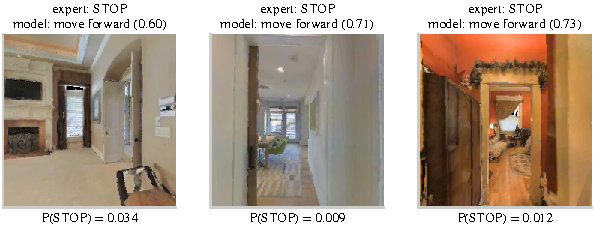
\includegraphics[width=0.72\linewidth]{figures/p1_stop_moments.pdf}
  \caption{\textbf{The selected checkpoint at the goal.} The selection set has three \textsc{stop}
  decisions, and all three are shown. The checkpoint is the one the
  selection rule picks, update $160$ of unweighted seed $20260826$. It emits \textsc{move\_forward} at all three, with probability
  $0.60$ to $0.73$, giving \textsc{stop} between $0.009$ and $0.034$. Images are Habitat-Sim renders
  of Matterport3D scans, and no physical robot was used. Cross-entropy stays low because these are three decisions
  in $256$.}
  \label{fig:stop_moments}
\end{figure}

\begin{figure}[t]
  \centering
  \begin{minipage}[c]{0.490\linewidth}\centering
    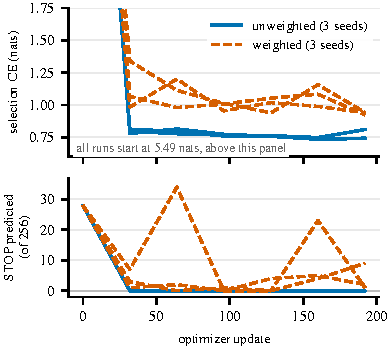
\includegraphics[width=\linewidth]{figures/p1_blind_metric.pdf}
  \end{minipage}\hfill
  \begin{minipage}[c]{0.475\linewidth}
  \caption{\protect\raggedright\textbf{The selection loss falls while the unweighted runs stop
  predicting \textsc{stop}.} Cross-entropy on the frozen selection set, and how many of those $256$ decisions
  the model calls \textsc{stop}. Solid is unweighted, dashed weighted, three seeds each.
  Unweighted cross-entropy falls to about $0.8$ within $32$ updates and flattens while predicted
  \textsc{stop} goes from $28$ to zero and never returns. The weighted runs stay between $0.92$ and
  $1.34$, and their predicted \textsc{stop} spikes to $34$ and $23$ at isolated points.}
  \label{fig:blind_metric}
  \end{minipage}
\end{figure}
